\section{Тестирование.}

\begin{figure}[ht]
    \begin{center}
        \includegraphics[width=0.5\textwidth]{../resources/imageNoised}
    \end{center}
    \caption{Изначальное изображение.}
\end{figure}

\begin{figure}[ht]
    \begin{center}
        \includegraphics[width=0.5\textwidth]{../resources/outputDefault}
    \end{center}
    \caption{Результат со стандартными параметрами.}
\end{figure}

\begin{figure}[ht]
    \begin{center}
        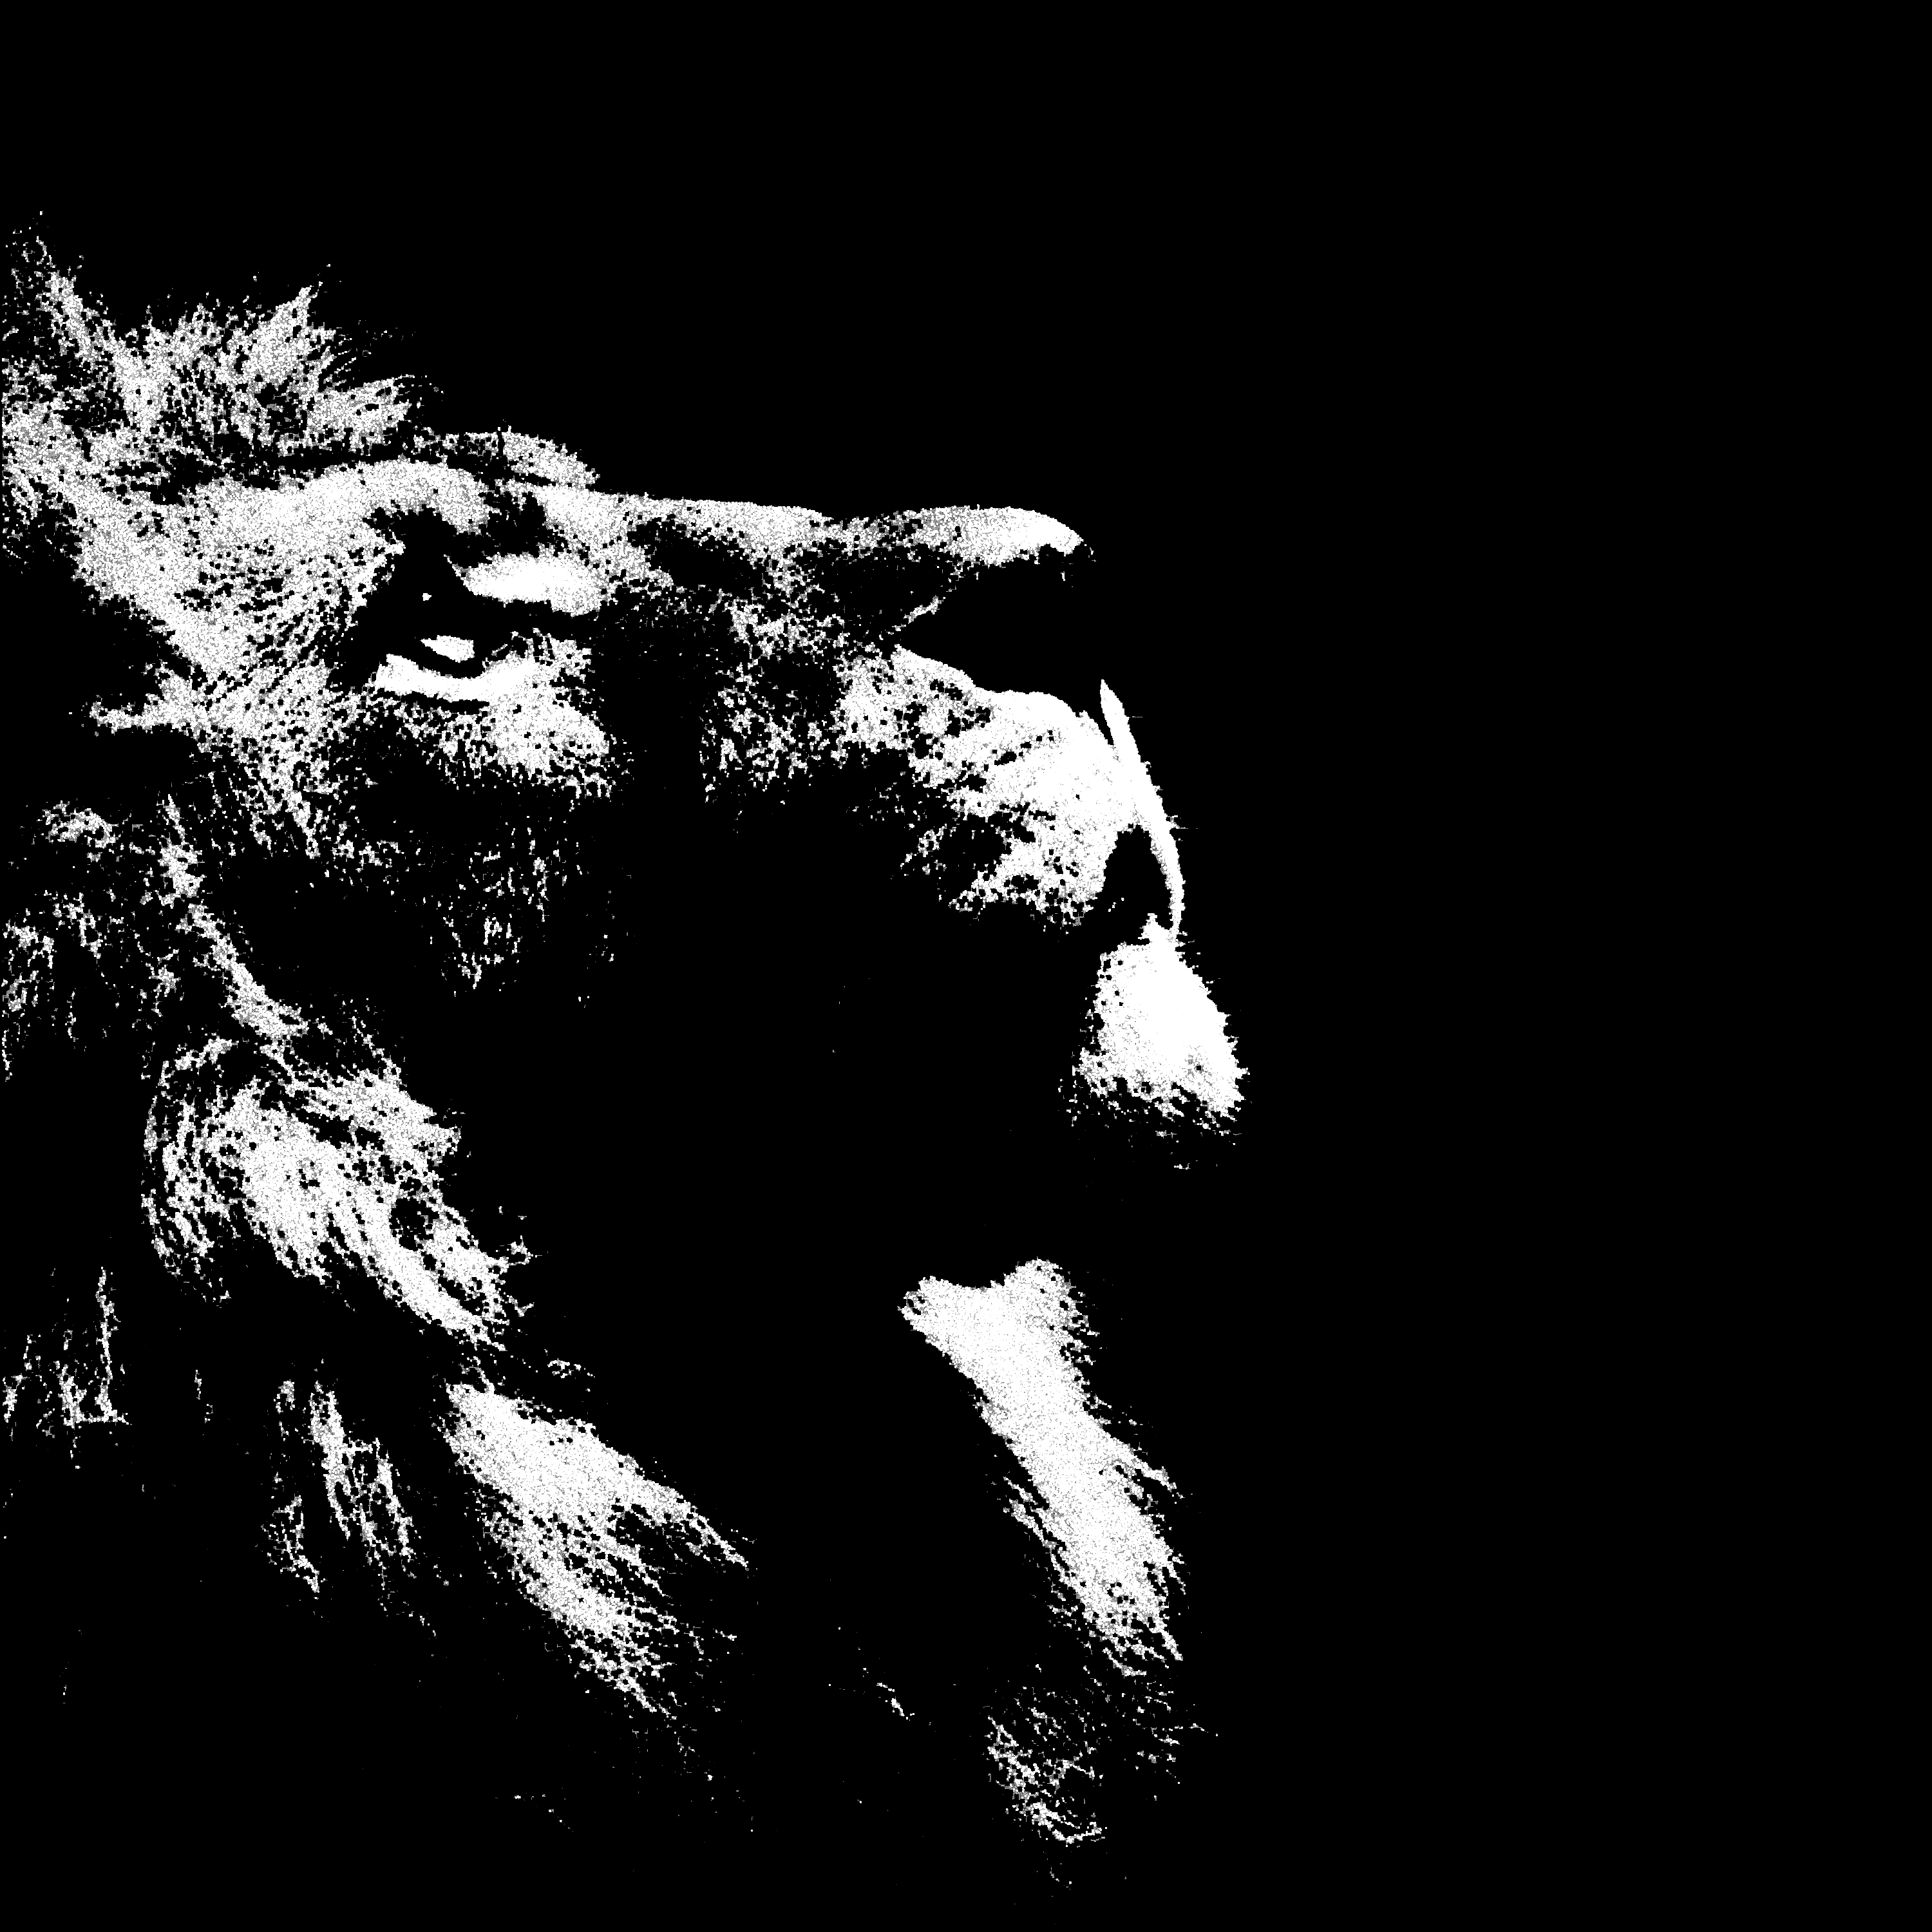
\includegraphics[width=0.5\textwidth]{../resources/outputNoDenoise}
    \end{center}
    \caption{Результат без удаления шумов.}
\end{figure}

\begin{figure}[ht]
    \begin{center}
        \includegraphics[width=0.5\textwidth]{../resources/outputNoUpgrade}
    \end{center}
    \caption{Результат без улучшения.}
\end{figure}

\begin{figure}[ht]
    \begin{center}
        \includegraphics[width=0.5\textwidth]{../resources/outputNoIncreace}
    \end{center}
    \caption{Результат без увеличения.}
\end{figure}

\begin{figure}[ht]
    \begin{center}
        \includegraphics[width=0.5\textwidth]{../resources/outputNoReduce}
    \end{center}
    \caption{Результат без уменьшения.}
\end{figure}

\begin{figure}[ht]
    \begin{center}
        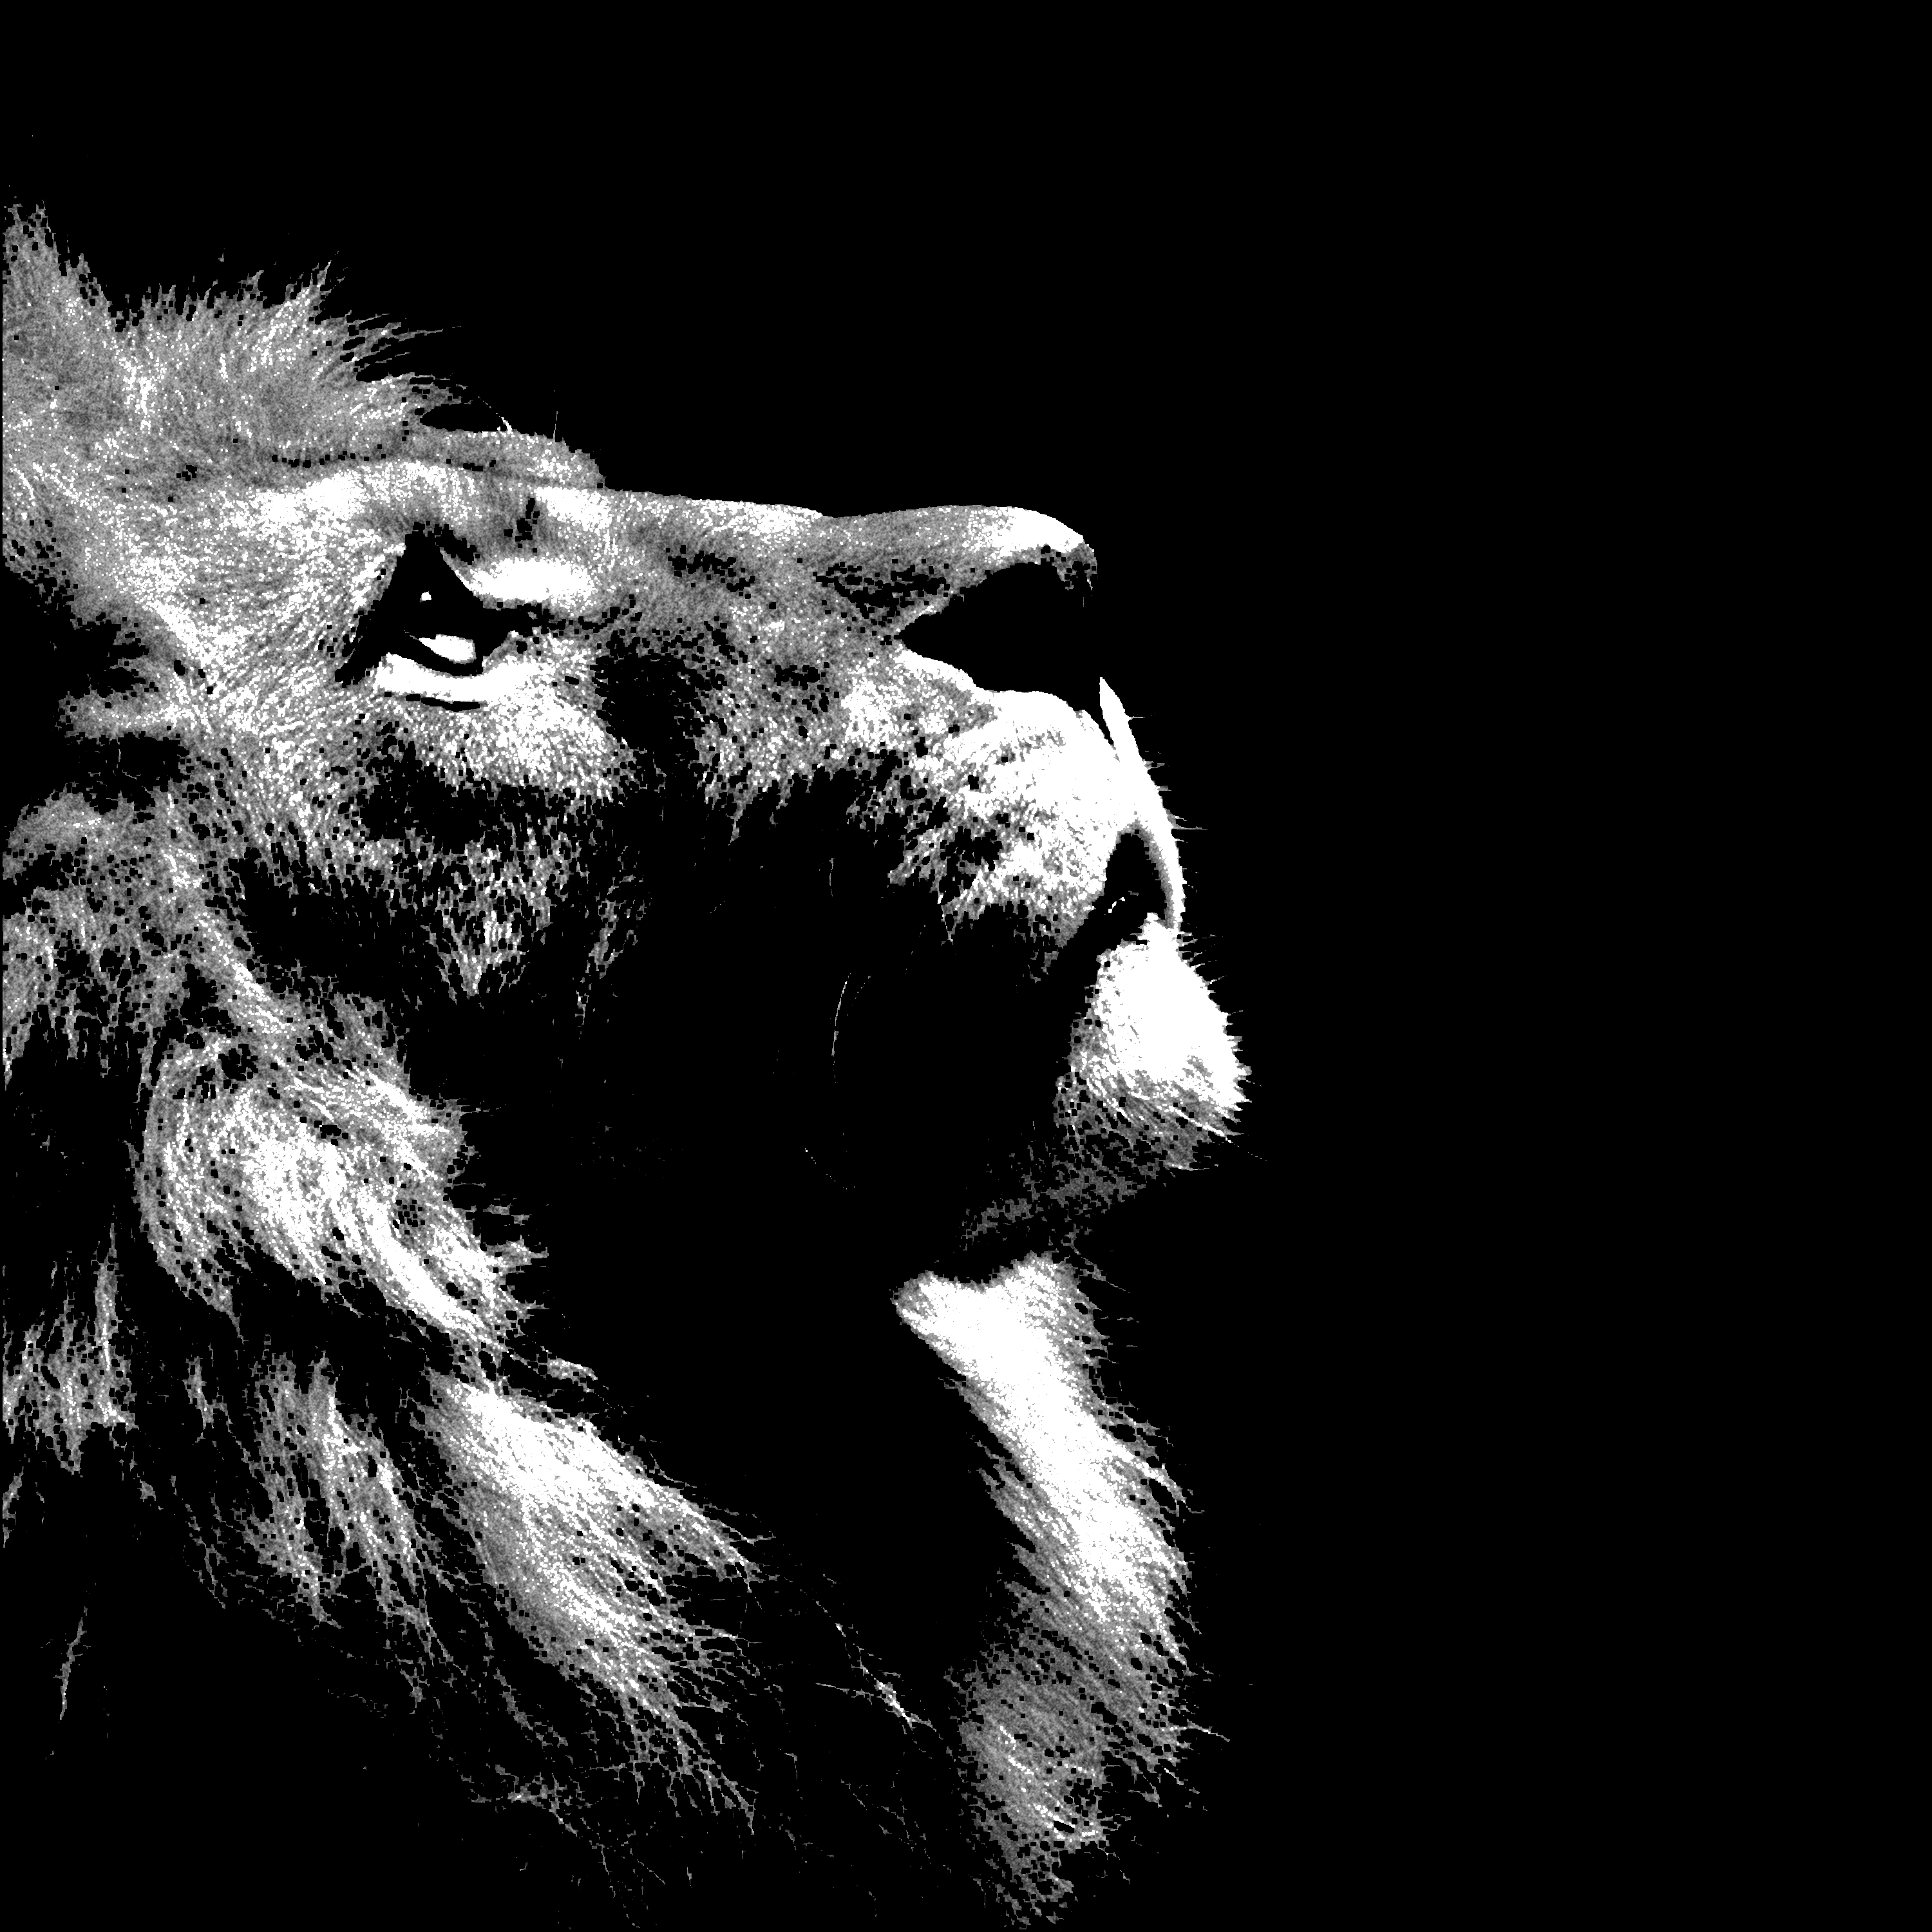
\includegraphics[width=0.5\textwidth]{../resources/outputStrongUpgrade}
    \end{center}
    \caption{Результат со смягчением порогов увеличения/уменьшения.}
\end{figure}

\begin{figure}[ht]
    \begin{center}
        \includegraphics[width=0.5\textwidth]{../resources/output3threads}
    \end{center}
    \caption{Результат на трёх потоках.}
\end{figure}

\begin{figure}[ht]
    \begin{center}
        \includegraphics[width=0.5\textwidth]{../resources/output6threads}
    \end{center}
    \caption{Результат на шести потоках.}
\end{figure}

\begin{figure}[ht]
    \begin{center}
        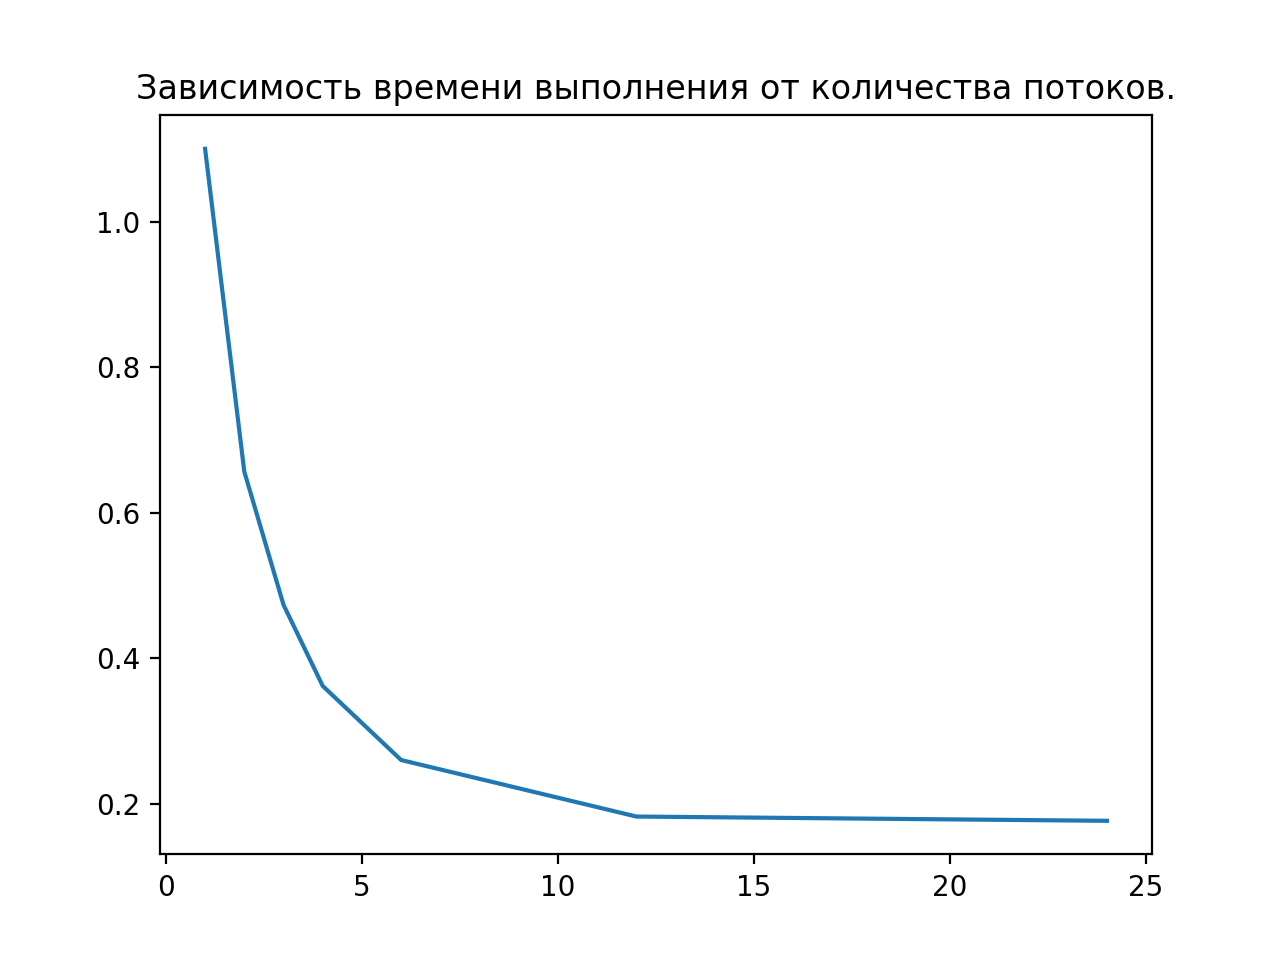
\includegraphics[width=0.9\textwidth]{../resources/graph}
    \end{center}
    \caption{Результат на шести потоках.}
\end{figure}

На моей машине 12 потоков.
Поэтому на значениях больше 12 роста нет.